\documentclass[main]{subfiles}


\title[AutoML in the Age of Foundation Models]{AutoML in the Age of Foundation Models}
\subtitle{Prior-fitted networks for Hyperparameter Optimization}
\author[Marius Lindauer]{Marius Lindauer}
\date{}

\titlebackground*{images/AutoML_Agentic}

%\institute{}
%\date{}

\begin{document}
	
	\maketitle
	

%----------------------------------------------------------------------
%----------------------------------------------------------------------
\begin{frame}[c]{Recap: What is TabPFN? \liturl{Hollmann et. 2022}{https://arxiv.org/abs/2207.01848} \liturl{Hollmann et al. 2024}{https://www.nature.com/articles/s41586-024-08328-6}}

\centering
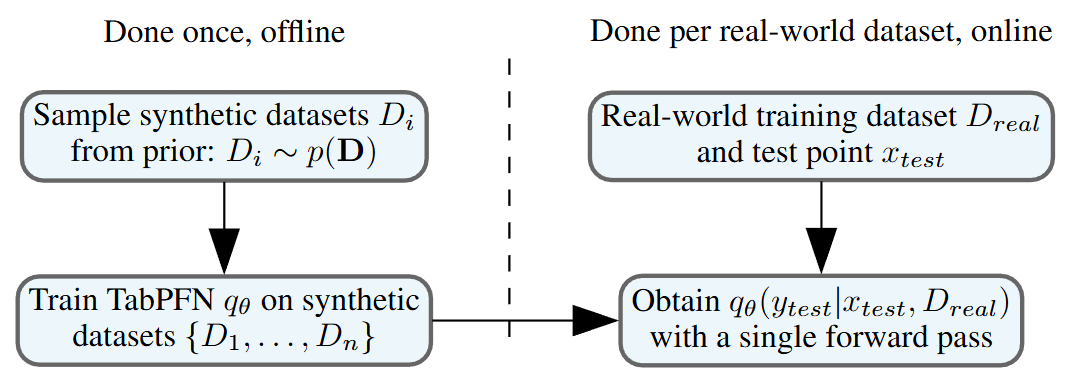
\includegraphics[width=0.8\textwidth]{images/tabpfn_overview}

\end{frame}
%-----------------------------------------------------------------------
%-----------------------------------------------------------------------
\begin{frame}{1. Overview: PFNs as BO Surrogates \liturl{Müller et al. 2023}{https://arxiv.org/abs/2305.17535}}
    \begin{itemize}
        \item \textbf{Core Idea:} Replace Gaussian Processes (GPs) fitted via Empirical Bayes with \textbf{Prior-data Fitted Networks (PFNs)}.
        \item \textbf{In-Context Learning:} PFNs act as a surrogate model that approximates the Posterior Predictive Distribution in a single forward pass.
        \item \textbf{Key Shift:}
            \begin{itemize}
                \item \textit{Traditional BO:} Fit model parameters (e.g., GP lengthscales) to history $D_k$ at every step (online cost).
                \item \textit{PFN BO:} Pre-train a Transformer on a prior distribution once (offline cost), then inference is instant.
            \end{itemize}
        \item \textbf{Benefit:} Enables complex priors (e.g., BNNs) and custom extensions (user priors) that are analytically intractable for standard GPs.
    \end{itemize}
\end{frame}

%----------------------------------------------------------------------
%----------------------------------------------------------------------
\begin{frame}{PFN Training: Learning the Prior}
    \begin{itemize}
        \item \textbf{Objective:} Train a Transformer model to mimic Bayesian inference for a specific prior source $p(\mathcal{D})$.
        \item \textbf{Process:}
            \begin{enumerate}
                \item Sample synthetic datasets $\hist = \{(\conf_i, \cost_i)\}_{i=1}^n$ from the prior (e.g., GP, BNN, HEBO priors).
                \item Split $D$ into training set $D_{train}$ and test query $(\conf_{test}, \cost_{test})$.
                \item Minimize the cross-entropy loss (approximation of Posterior Predictive Distribution):
                $$ \mathcal{L}(\theta) = \mathbb{E}_{D \sim p(\mathcal{D})} \left[ -\log q_{\theta}(\cost_{test} | \conf_{test}, D_{train}) \right] $$ 
            \end{enumerate}
        \item \textbf{Output Distribution:} Uses a \textbf{Riemann distribution} (discretized buckets) to model arbitrary, potentially multi-modal posterior shapes.
    \end{itemize}
\end{frame}

%----------------------------------------------------------------------
%----------------------------------------------------------------------
\begin{frame}{Learning Curve Predictions with TabPFN \liturl{Rakotoarison et al. 2024}{https://arxiv.org/abs/2404.16795}} 

\centering
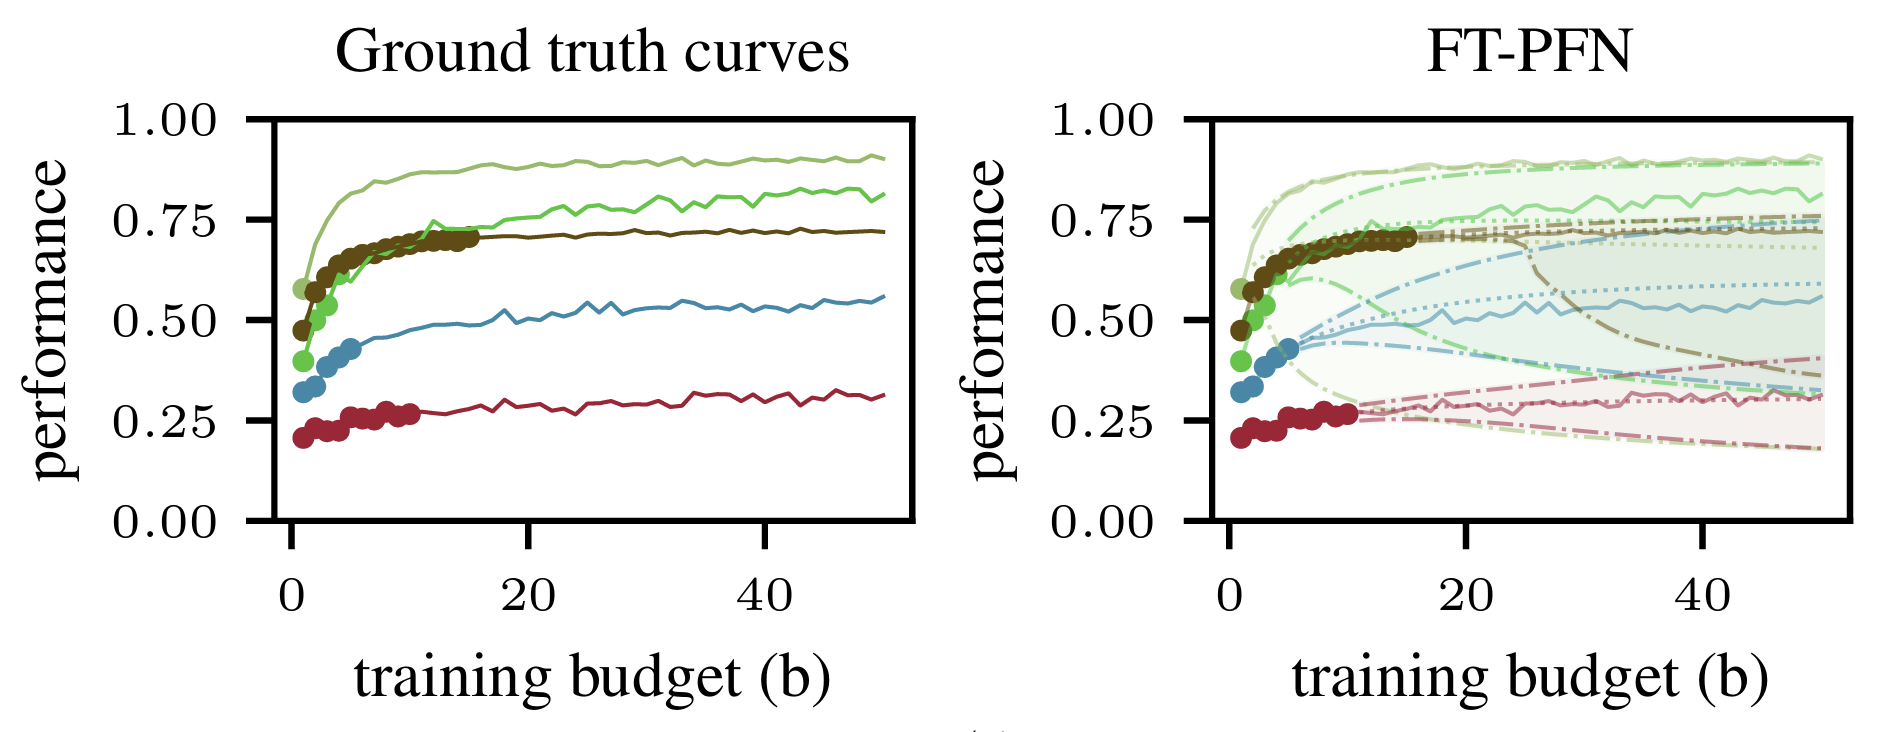
\includegraphics[width=1\textwidth]{images/ifbo_curves.png}

\end{frame}
%----------------------------------------------------------------------
%----------------------------------------------------------------------
\begin{frame}{FT-PFN: In-Context Learning for Learning Curves\\ \liturl{Rakotoarison et al. 2024}{https://arxiv.org/abs/2404.16795}}

    \begin{itemize}
        \item \textbf{Core Idea:} Replace online surrogate training with a Transformer-based \textbf{PFN} that performs Bayesian inference via In-Context Learning (ICL) in a single forward pass.
        \item \textbf{Meta-Training via Synthetic Prior:} 
        The model is trained offline on millions of synthetic \textbf{learning curves} generated by a structural prior, $\pi_{curve}$ %, which mimics real HPO behaviors (saturation, divergence).
        
        \item \textbf{Generative Process (The Prior):}
        Performance $\cost_t$ at time $t$ for config $\conf$ is modeled as a weighted combination of basis functions (e.g., Power Law, Hill):
        $$ \pi_{curve}(\conf, t) \sim \mathcal{N}\left(\cost_0 + (\cost_{\infty} - \cost_0) \sum_{k=1}^K w_k f_k(t; \Psi_k), \sigma^2\right) $$
        where parameters $\sigma^2$ (variance of normal distr.), $\cost_{\infty} \text{(final performance)},$ $\Psi \text{(basis function)},$ $w \text{ (weight of basis function)}$ are sampled from a randomized neural network $\pi_{config}(\conf)$. $\cost_0$ is assumed to be independent of $\conf$.

        % \item \textbf{Inference:}
        % Given history $H$ (partial curves), FT-PFN approximates the Posterior Predictive Distribution (PPD) without gradient updates:
        % $$ q_\theta(\lambda_{target}, H) \approx \mathbb{P}(y_{target} | H, \lambda_{target}) $$
        % \textit{Benefit:} 10-100x faster than Deep Ensembles/GPs; no hyper-hyperparameters.
    \end{itemize}
\end{frame}

%----------------------------------------------------------------------

%----------------------------------------------------------------------
\begin{frame}{ifBO Framework \& MFPI-random Acquisition\\ \liturl{Rakotoarison et al. 2024}{https://arxiv.org/abs/2404.16795}}

    \begin{itemize}
        \item 
    \textbf{Freeze-Thaw BO:} Dynamically allocates budget increments to configurations, i.e., pausing and resuming based on predicted potential.
        \item \textbf{MF-PI-random:} A parameter-free acquisition that randomizes the horizon and threshold at \textit{every} step to hedge risks (portfolio effect).
        $$ \alpha(\conf) = \mathbb{P}\left( \mathcal{M}(\conf, \min(b_{\conf} + h^{rand}, b_{max})) > T^{rand} \right) $$
        \begin{itemize}
            \item \textbf{Horizon:} $h^{rand} \sim \mathcal{U}(1, b_{max})$ (short vs. long-term gains)
            \item \textbf{Threshold:} $T^{rand} = f_{best} + 10^{\tau} \cdot (1 - f_{best})$, where $\tau \sim \mathcal{U}(-4, -1)$ (explore vs exploit)
        \end{itemize}

        \item \textbf{The ifBO Loop:} 
        \begin{enumerate}
            \item Context $H \to$ FT-PFN (In-Context) $\to$ Posterior Predictive Distribution. 
            \item Sample $h^{rand}, T^{rand}$ and select $\conf^* \in \arg\max \alpha(\conf)$. 
            \item Thaw $\conf^*$ for 1 step; update $H$.
        \end{enumerate}
    \end{itemize}
\end{frame}
\begin{frame}{Summary} 

Most important insights from this video:

\begin{enumerate}
    \item PFNs can be pre-trained on BO-like data
    \item Pre-trained PFNs can be used to as efficient surrogate models
    \item PFNs can be used to model learning curves, giving rise to multi-fidelity HPO with a single pre-trained model
\end{enumerate}


\end{frame}

\end{document}

